\documentclass[a4paper,12pt]{article}

\usepackage[utf8]{inputenc}
\usepackage[left=0.5in,right=0.5in,top=1in,bottom=1in]{geometry}
\usepackage{amsmath,amssymb,amsfonts}
\usepackage{pgfplots,graphicx,calc,changepage}
\pgfplotsset{compat=newest}
\usepackage{enumitem}
\usepackage{fancyhdr}
\usepackage[colorlinks = true, linkcolor = blue]{hyperref}

% Syntax highlighting
\usepackage{listings}
\usepackage{xcolor}

\definecolor{codegreen}{rgb}{0.40,0.62,0.07}
\definecolor{codegray}{rgb}{0.5,0.5,0.5}
\definecolor{codeblue}{rgb}{0.09,0.57,0.73}
\definecolor{backcolour}{rgb}{1,1,1}

\lstdefinestyle{mystyle}{
    backgroundcolor=\color{backcolour},   
    commentstyle=\color{codegreen},
    keywordstyle=\color{magenta},
    numberstyle=\tiny\color{codegray},
    stringstyle=\color{codeblue},
    basicstyle=\ttfamily\small,
    breaklines=true,                     
    keepspaces=true,                 
    numbers=left,                    
    numbersep=5pt,                  
    showspaces=false,
    showstringspaces=false,
    showtabs=false,                  
    tabsize=4
}

\lstset{style=mystyle}

\newcommand{\nats}{\mathbb{N}}
\newcommand{\reals}{\mathbb{R}}
\newcommand{\rats}{\mathbb{Q}}
\newcommand{\ints}{\mathbb{Z}}
\newcommand{\comps}{\mathbb{C}}
\newcommand{\pols}{\mathcal{P}}
\newcommand{\cants}{\Delta\!\!\!\!\Delta}
\newcommand{\eps}{\varepsilon}
\newcommand{\st}{\backepsilon}
\newcommand{\abs}[1]{\left| #1 \right|}
\newcommand{\dom}[1]{\mathrm{dom}\left(#1\right)}
\newcommand{\for}{\text{ for }}
\newcommand{\dd}[1]{\mathrm{d}#1}
\newcommand{\spn}{\mathrm{sp}}
\newcommand{\nul}{\mathcal{N}}
\newcommand{\col}{\mathrm{col}}
\newcommand{\rank}{\mathrm{rank}}
\newcommand{\norm}[1]{\lVert #1 \rVert}
\newcommand{\inner}[1]{\left\langle #1 \right\rangle}
\newcommand{\pmat}[1]{\begin{pmatrix} #1 \end{pmatrix}}
\renewcommand{\and}{\text{ and }}

\newsavebox{\qed}
\newenvironment{proof}[2][$\square$]
    {\setlength{\parskip}{0pt}\par\textit{Proof:} #2\setlength{\parskip}{0.25cm}
        \savebox{\qed}{#1}
        \begin{adjustwidth}{\widthof{Proof:}}{}
    }
    {
        \hfill\usebox{\qed}\end{adjustwidth}
    }

\pagestyle{fancy}
\fancyhead{}
\lhead{Caleb Jacobs}
\chead{APPM 5600: Numerical Analysis I}
\rhead{Homework \#10}
\cfoot{}
\setlength{\headheight}{35pt}
\setlength{\parskip}{0.25cm}
\setlength{\parindent}{0pt}

\begin{document}
\section*{Problems}
\begin{enumerate}[label = \arabic*.]
	\item Consider the error plot and surface plots below comparing regular a regular 2D Lagrange interpolant vs a Boolean Sum Lagrange based interpolant
	\begin{figure}[h!]
		\centering
		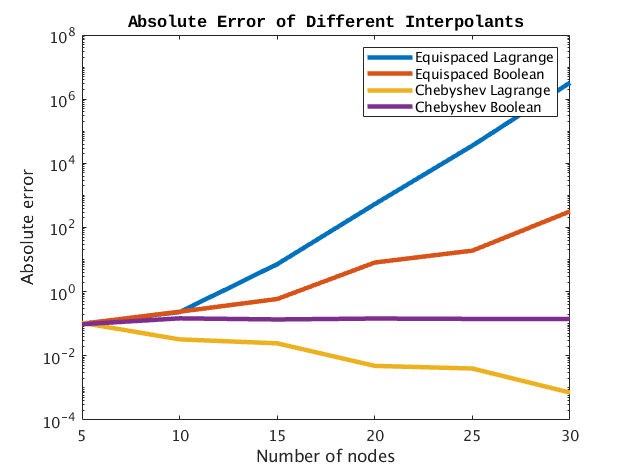
\includegraphics[width = 0.6\textwidth]{images/Errors.png}
		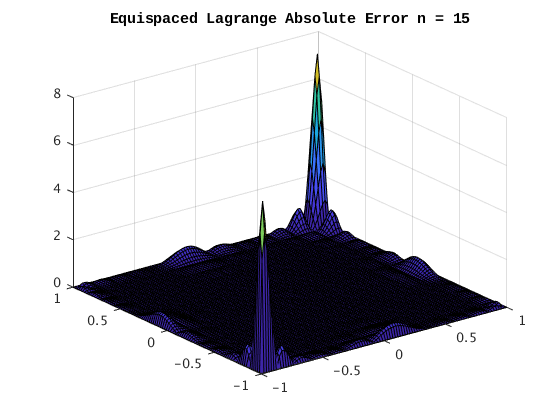
\includegraphics[width = 0.45\textwidth]{images/EL15.png}
		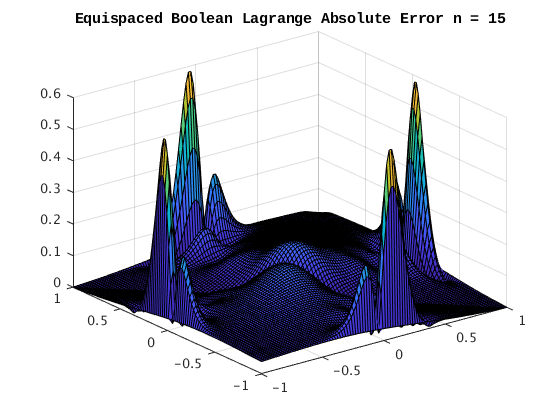
\includegraphics[width = 0.45\textwidth]{images/EB15.png} \\
		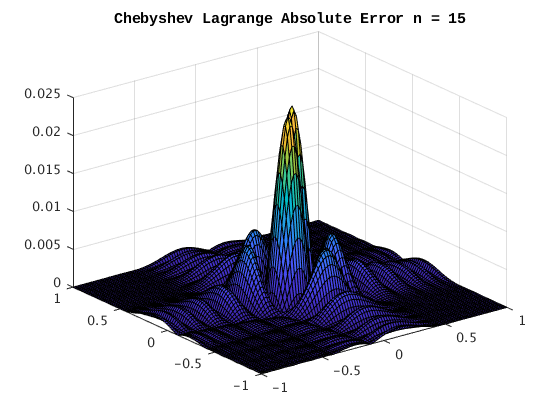
\includegraphics[width = 0.45\textwidth]{images/CL15.png}
		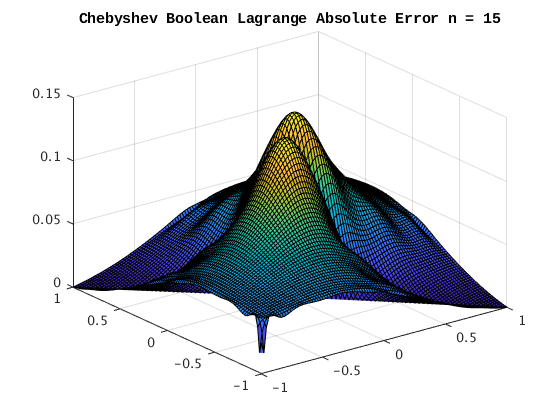
\includegraphics[width = 0.45\textwidth]{images/CB15.png}
	\end{figure}

	\newpage
	\begin{enumerate}[label = (\alph*)]
		\item From the error plot focusing on the equispaced curves, we can see that using a Boolean Sum Lagrange Interpolant works marginally better than a regular Lagrange based method. Although both errors are increasing as the number of nodes increases, the Boolean Sum is increasing a much slower rate.
		
		\item From the same error but now focusing on the Chebyshev a curves, we see a slightly different trend. Now the error in the Boolean Sum is remaining relatively constant with an increase in the number of nodes while the error is actually decreasing for the regular Lagrange interpolant.
		 
		\item To understand the differences between the two methods, let's take a closer look at the sums we have to compute in each method. In the case of the regular Lagrange basis, we experience Runge at the boudnaries of our interval due to the Lagrange polynomials. So, using Chebyshev nodes pushes the error to the inside of the interval allowing us to actually have convergence of the Lagrange interpolant. Furthermore, the Lagrange interpolant uses the lagrange basis over our whole domain which pushes the error to the corners of our boundaries.
		
		On the other hand, we have the Boolean Sum Lagrange interpolant which relies on the data along each x and y axis individually instead of having all of the cross terms. This splitting of the data causes the error to be focused near the middle of our boundaries. So, using Chebyshev nodes, the error is mitigated at the boundaries but the Runge at the middle of the boundaries was not bad to begin with so the error doesn't change much.
	\end{enumerate}
	
	\item Prove the following result: Let $ f \in C^2 [a,b] $ with $ f''(x) > 0 $ for $ a \leq x \leq b $. If $ q_i^*(x) = a_0 + a_1 x $ is the linear minimax approximation to $ f(x) $ on $ [a,b] $, then 
	\[
		a_1 = \frac{f(b) - f(a)}{b - a}, \quad a_0 = \frac{f(a) + f(c)}{2} - \frac{a + c}{2} \cdot \frac{f(b) - f(a)}{b - a}
	\]
	where $ c $ is the unique solution of
	\[
		f'(c) = \frac{f(b) - f(a)}{b - a}.
	\]
	
	\begin{proof}{}
		From Cauchy's Equioscillation Theorem, we know there exists a unique polynomial of the form $ p_1^*(x) = a_0+ a_1 x $ such that the error $ E(x) = f(x) - p_1^*(x) $ satisfies
		\begin{align}
			E(a) &= \rho \label{equ:1} \\
			E(c) &= -\rho \label{equ:2} \\ 
			E(b) &= \rho \label{equ:3} \\
			E'(c) &= 0 \label{equ:4}
		\end{align}
		where $ \rho $ is the maximum error on $ [a, b] $ and $ c \in (a,b) $. Now using \eqref{equ:4}, we have
		\[
			E'(c) = f'(c) - a_1 = 0 \implies a_1 = f'(c).
		\]
		Then, (\eqref{equ:1} - \eqref{equ:3}) implies
		\[
			f(a) - f(b) + a_1(b - a) = 0 \implies \boxed{a_1 = \frac{f(b) - f(a)}{b - a}}
		\]
		which implies $ c $ is the solution to 
		\[
			\boxed{f'(c) = \frac{f(b) - f(a)}{b - a}}.
		\]
		Next, (\eqref{equ:1} + \eqref{equ:2}) implies
		\[
			f(a) + f(c) - 2a_0 - a_1 (a + c) = 0 \implies \boxed{a_0 = \frac{f(a) + f(c)}{2} - \frac{a + c}{2} \cdot \frac{f(b) - f(a)}{b - a}}.
		\]
		Finally, the max error can be obtained from \eqref{equ:1} as
		\[
			\boxed{\rho = f(a) - \frac{f(a) + f(c)}{2} + \frac{f(b) - f(a)}{b - a} \left(\frac{a + c}{2} -  a\right)}.
		\]
	\end{proof}
\end{enumerate}

\section*{Code used}
\rule{\textwidth}{4pt}
	\lstinputlisting[language = matlab]{code/Problem_1.m}
\rule{\textwidth}{4pt}

\end{document}